
%heti uusiks selitys
sovelluksen ominausiitta haluttiin muokata
Sovelluksessa oli ominaisuus nimeltä progressio. kun käyttäjää luodaan voidaan antaa sille seurattava arvo. tämä voi olla esim kg, unenmäärä jne
käyttäjä voi sitten käyttöliittymästä lisätä arvoja. ja nähdä ne graafista. 
Tällä hetkellä käyttäjällä voi olla vain yksi seurattava arvo ja ominaisuutta haluttiin jatkojalostaa lisäämällä mahdollisuus usealla seurattavalle arvolle. 


\subsection*{selitys featuresta}
%  en tiedä pitäisikö selitys featuresta selittää mitä pitää tehdä. tuntuu että tämä pitäisi olla metatekstissä jos jotain...

Käyttäjien schemassa on arvo measurableThing joka pitäisi muuttaa listaksi. Tämä vaatii user schaman muuttamista.
Pitää myös lisätä mahdollisuus käyttäjien luonnissa lisätä useampi mitattava asia.
käyttäjillä on progressio sivu, josta voidaan lisätä arvoja.
tähän pitää lisätä mahdollisuus määritellä mitä arvoa halutaan inputtaa.
graafia pitää muuttaa siten, että se voi näyttää usean mitattavan arvon.
\medskip

%kaikille kuville oikeet koot
% ja medskipit kuntoon

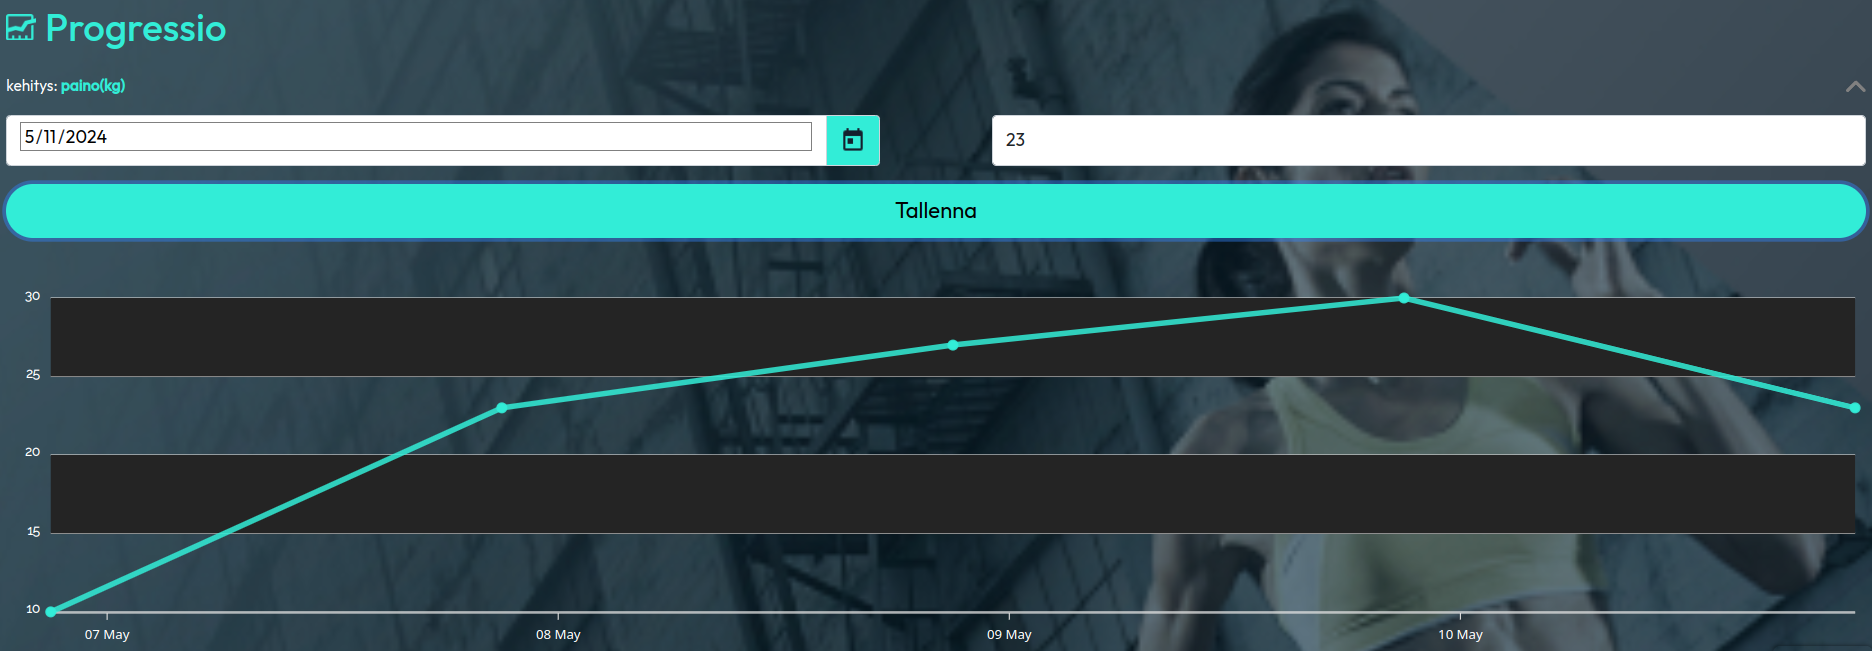
\includegraphics[width= 15cm, height=5cm]{src/public/progressiosingle.png} \\
kuvassa starttaamo progressio sivu alussa
\medskip

jotain tekstiä kuvasta 
eli paino tai kg ja input numerolle.
sitten graafi missä ne näkyy
\medskip


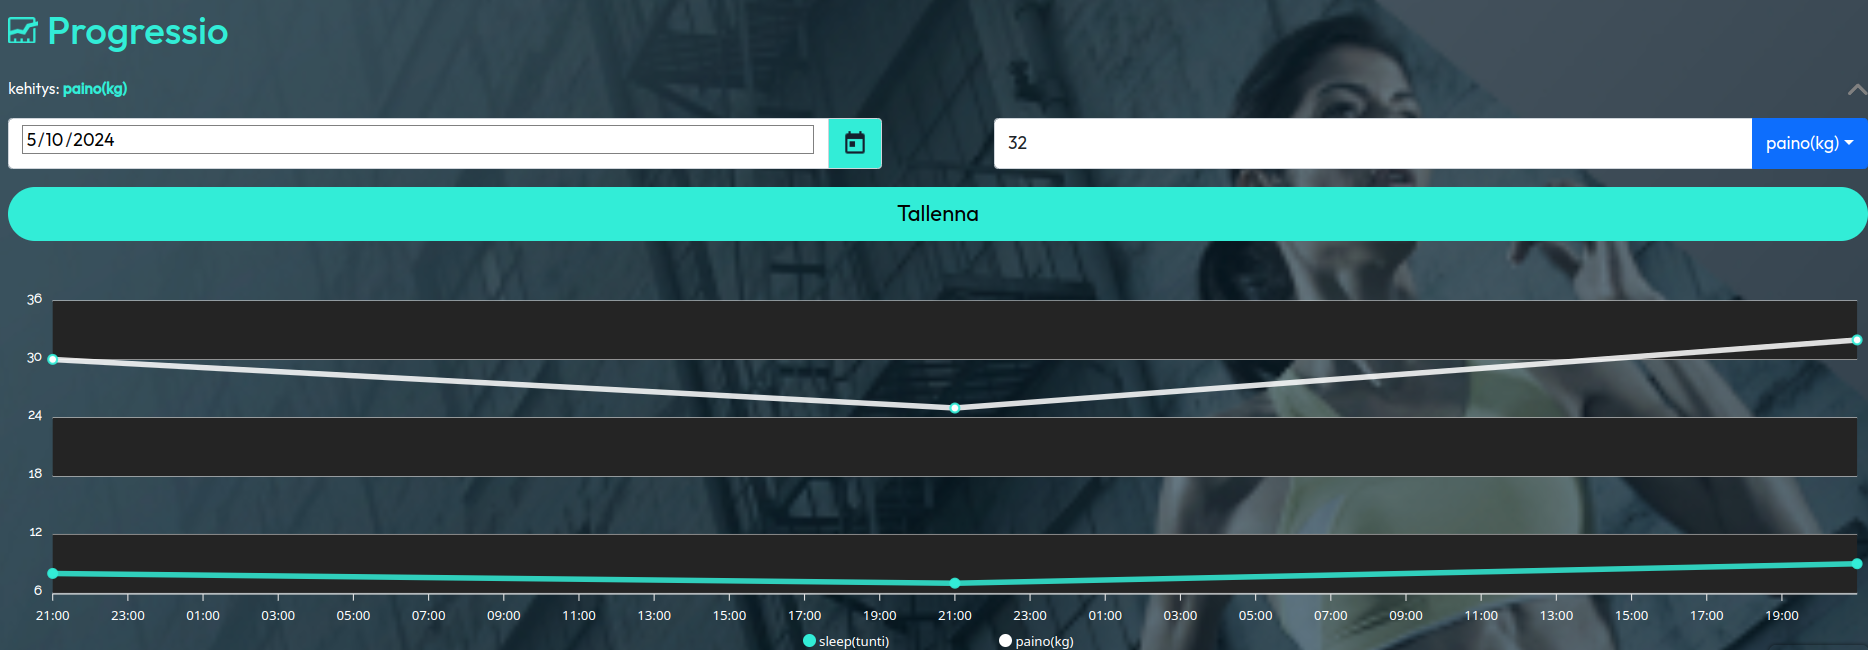
\includegraphics[width= 15cm, height=5cm]{src/public/progressmulti.png} \\
kuvassa starttaamo progressio sivu lopussa
\medskip


jotain tekstiä kuvasta 
eli paino tai kg ja input numerolle sitten on dropdown millä voi valitas.
sitten graafi missä ne kaikki näkyy
\medskip


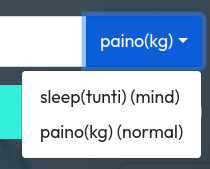
\includegraphics[width= 15cm, height=5cm]{src/public/progressselect.png} \\
progression laskuvalikko
\medskip


jotain lorem kuvasta.
voi valita mitä haluaa.
\medskip



\subsection*{user schema päivitys}

schema päivitys. measurableThing > measurableThings.  
rajapinnat on tyypitetty, joten pitää niitä muuttaa että voi toimia.
%jotain lisätekstiä rajapintojen tyypityksestä. ehkä jotain gql 
%
pitää muuttaa miten käyttöjiä luodaan. ja miten niitä päivitetään
pitää lisätä joku tapa millä lisätä useampia measurableThing eikä vain yhtä
\medskip

user migration. pitää migratoida kaikki aktiiviset asiakkaat measurableThings muotoon.
migraatio funktiot on sinänsä aika pelottavia sillä muutetaan kaikkien käyttäjien schemaa samaan aikaan. jos scheman muutoksessa tulee virhe meidän kaikki käyttäjät ovat scuffed.
funktion pitää olla luotettava ja sellainen että se toimii ekalla kerralla.
\medskip

\subsection*{toteutus}
%loppu kusee
graafin näyttämiseen käytetään reat apex charts kirjastoa. Kirjasto tukee useamman eroavan datan näyttämisen, joten uuden datan näyttäminen ei vaatinut muuta kun sen lisäämista graafiin.
react apex charts pystyi lisäämään vaan toisen seriessin. ja toimi melkein samantien
käyttöliuittymään pitää lisätä mahdollisuus siihen että valitaan mikä seurattavaa katsotaan
tähän taas laskuvalikko mihin vaan laitetaan kaikki jutut




\subsection*{yhteenveto}
miten meni ja miten onnistuin.
meni hyvin ominaisuus on nyt paikalla jne toimii jee.





